\chapter[\protect\vspace{-0.5ex}{VERY VERY VERY VERY VERY LONG TITLE I TEST THE DISPLAY IN THE HEADER}]{VERY VERY VERY VERY VERY LONG TITLE I TEST THE DISPLAY IN THE HEADER}
%Please keep the title in the toc and main content the same, don't use the feature to short the title, the purpose of applying the [] above is to decrease the vertical space between titles.
Refer to Appendix \ref{cha:appendix}.

\section{Section Test Example 1}

\begin{figure}[!hbp]
\begin{center}
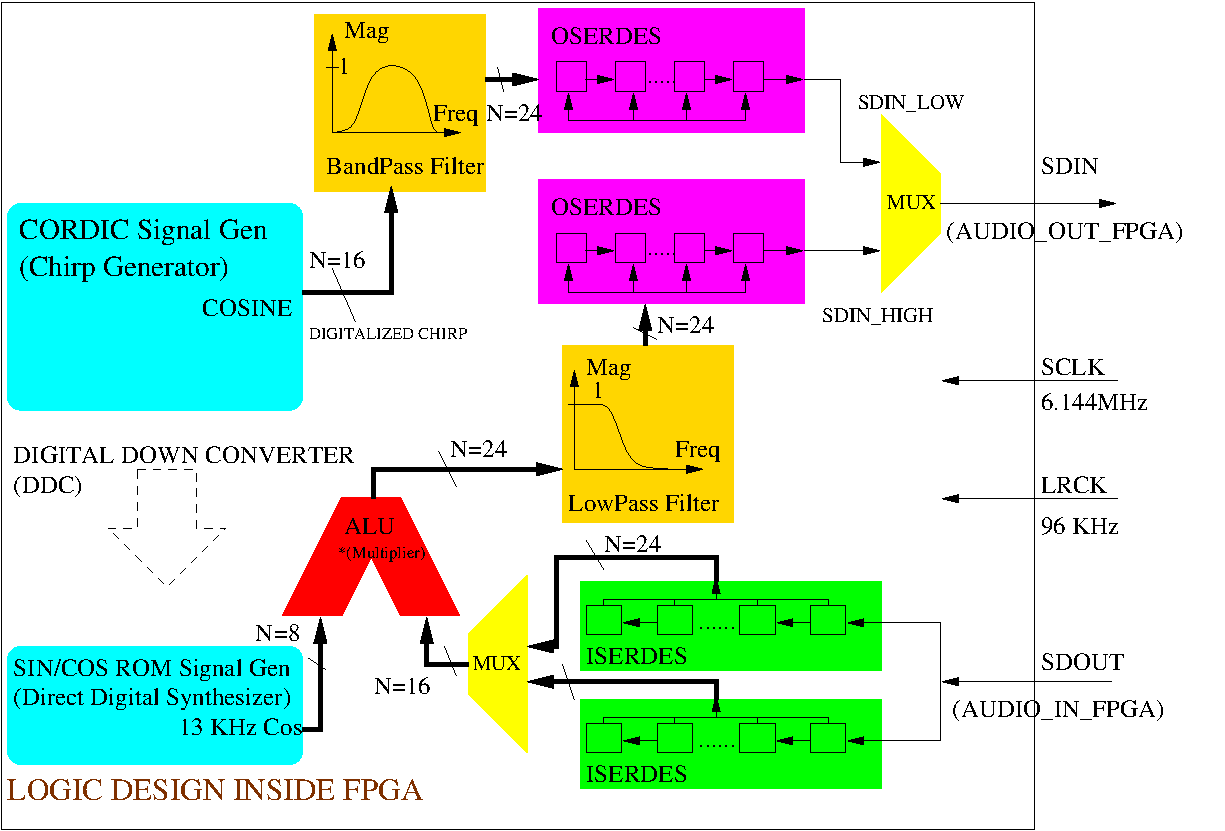
\includegraphics[width=\textwidth]{graphic/VERILOG_DESIGN_CHIRP.pdf}
\caption{Chapter 3 Figure Illustration Example }
\label{FPGAVerilogOverView}
\end{center}
\end{figure}

Fig \ref{FPGAVerilogOverView} is referred here.

\section{Test Section In This Chapter }
Section Title is to test toc display only, no actual meaning.
\subsection{Test Subsection In This Chapter}
 
 Picture/Table are only for illustration purpose, testing lof/lot, no exact meaning.
\begin{figure}[!hbp]
\begin{center}
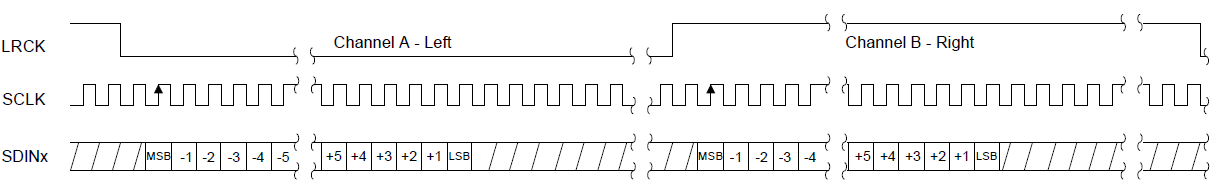
\includegraphics[width=\textwidth]{graphic/I2S_24Bit_Format.bmp}
\caption{$I^{2}S$ Random Pictures Showing Here For Test Purpose}
\label{fig:I2S_Timing}
\end{center}
\end{figure}


\subsection{Subsection Test Example 1}

\begin{figure}[!htbp]
\begin{center}
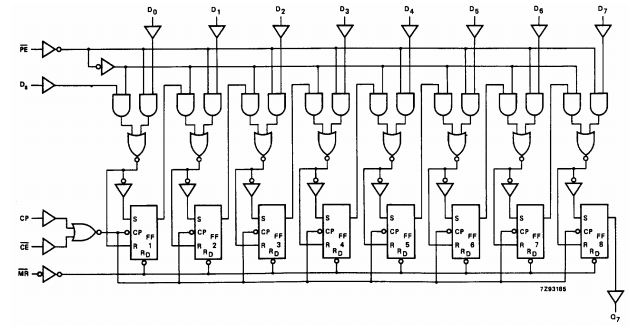
\includegraphics[width=\textwidth]{graphic/LogicDiagram_OSERDES.PNG}
\caption[\protect\vspace{-2.8ex}{This Is Another Example Of Long Figure/Table Title That Will Display As Single Spacing In The List Of Figures.}]{This Is Another Example Of Long Figure/Table Title That Will Display As Single Spacing In The List Of Figures.}
\label{fig:OSERDES}
\end{center}
\end{figure}



\section{Section Test Example 2}

 Fig \ref{FPGAVerilogOverView} are two practical implementations for the DDS framework.

\subsection{Subsection Test Example 2}

A chirp is a signal whose frequency increases (`up-chirp', Fig \ref{fig:upChirp} or decreases `down-chirp') with time. 

In a linear chirp, the instantaneous frequency $f(t)$ varies linearly with time, as shown in Equation \eqref{equ:linearChirp};
%
\begin{equation}
f(t)=f_0+k \cdot t \label{equ:linearChirp}
\end{equation}

$f_0$  is the starting frequency for sweeping in chirp. Its corresponding time domain function for a cosine linear chirp is;
%
\begin{equation}
x(t)=cos(2\pi \int_0^t f(t^{'})dt^{'})=cos(2\pi f_{0}t+k \pi t^2)  \label{equ:int_linearChirp}  
\end{equation}
%
%
\begin{figure}[!hbp]
\begin{center}
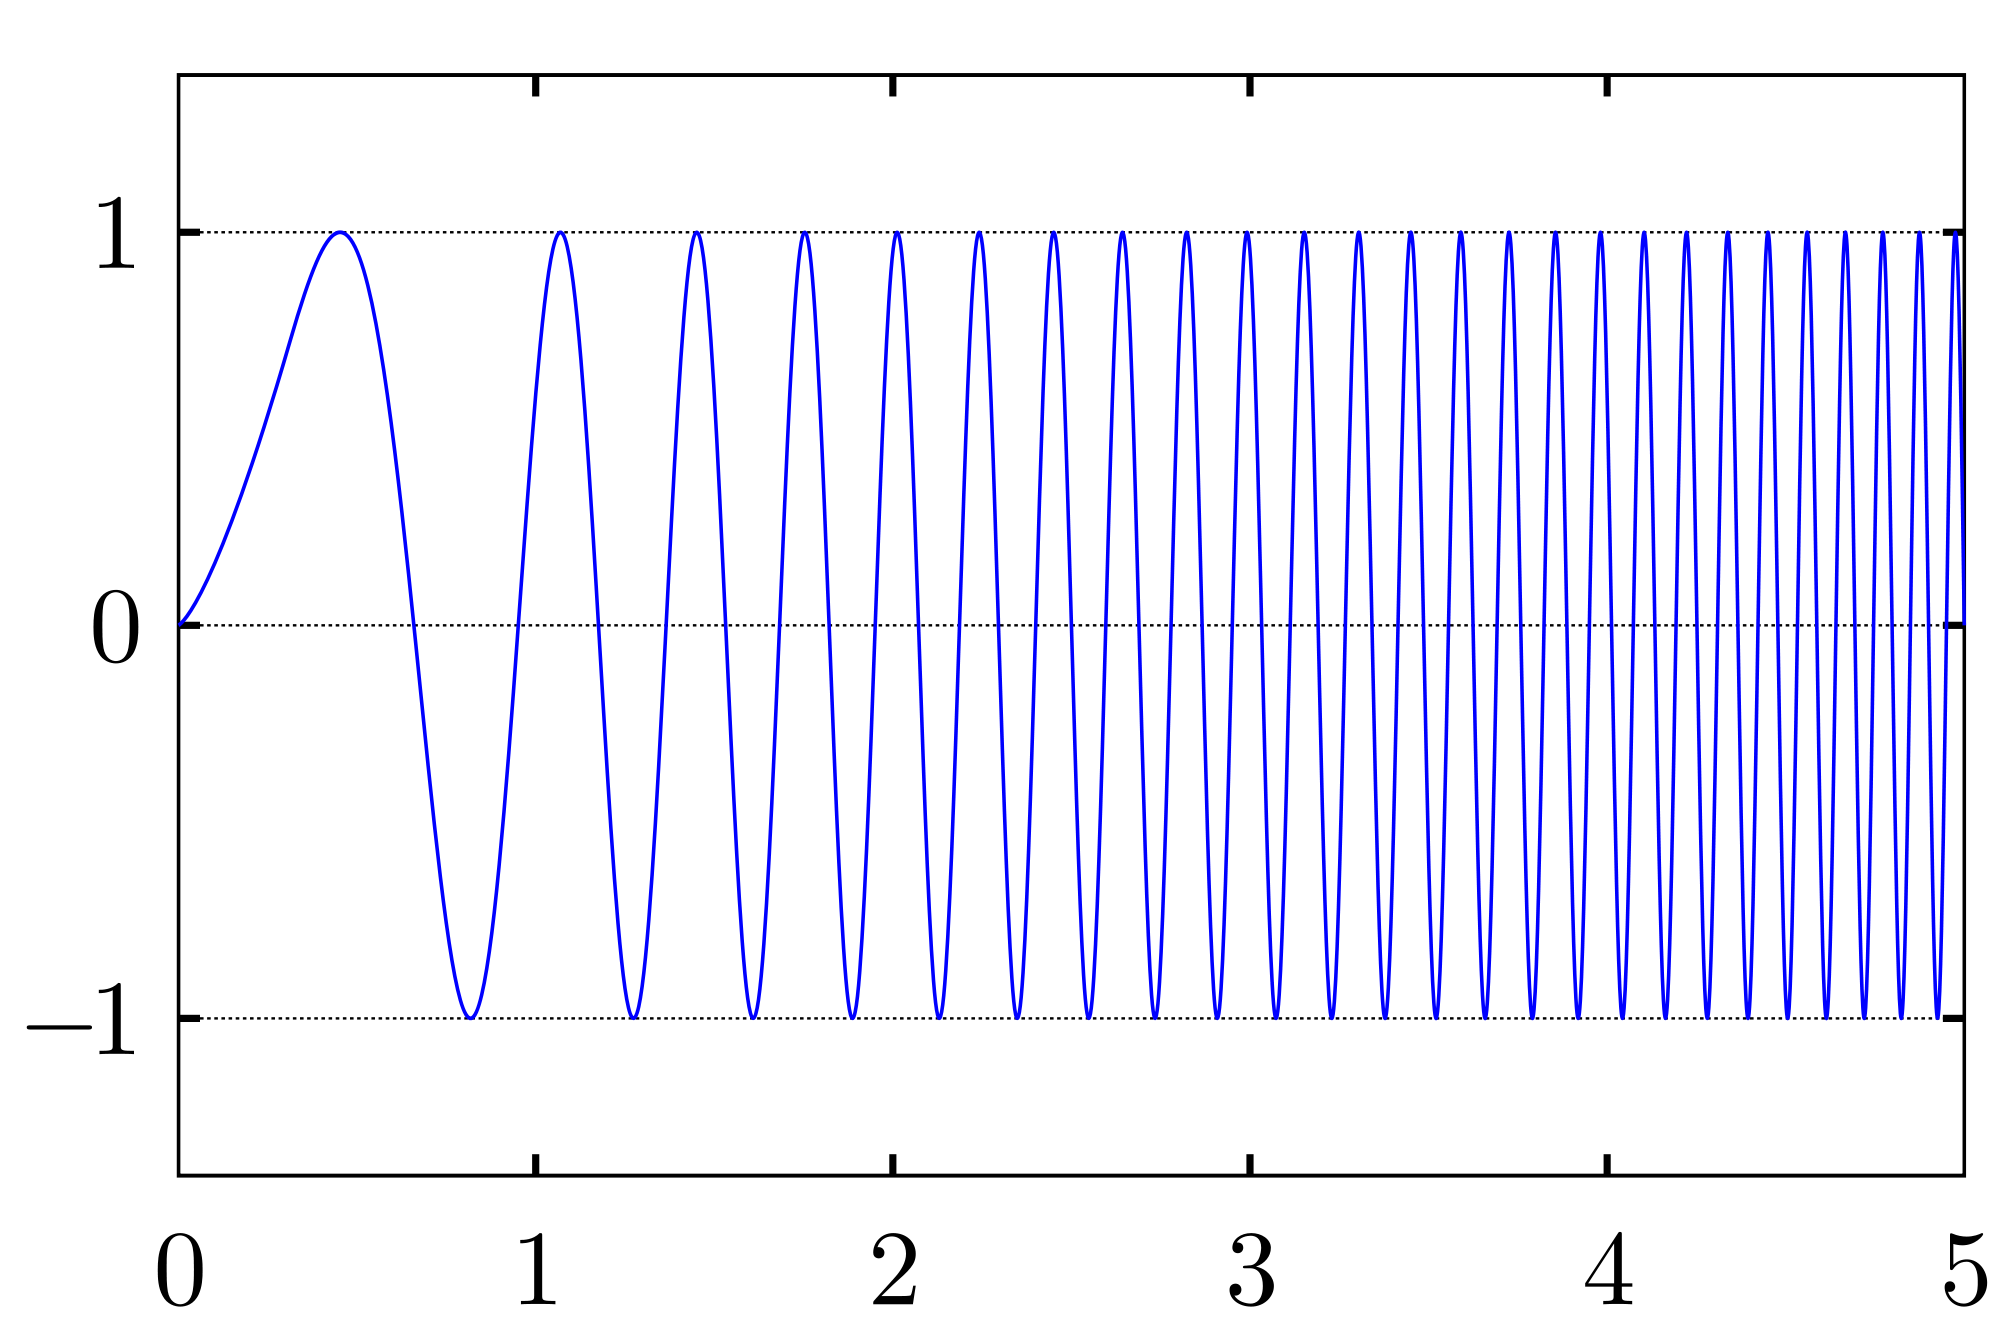
\includegraphics[width=0.8\textwidth]{graphic/2000px-Linear-chirp.svg.png}
\caption{Test Example Picture}
\label{fig:upChirp}
\end{center}
\end{figure}
The implementation of \ref{equ:int_linearChirp} could be simplified.
\subsection{Subsection Test Example 3}

\subsubsection{Subsubsection Test Example 1}
Example of multiple line \textbf{verbatim} environment.
\pagebreak[4]
\begin{verbatim}
      123
   x 	456
   ==========
     	738  (this is 123 x 6)
     615   (this is 123 x 5, shifted one position to the left)
   +492    (this is 123 x 4, shifted two positions to the left)
   =========
    56088
\end{verbatim}

\subsubsection{Subsubsection Test Example 2}
Example Equation is below in Equ. \eqref{equ:rotateVector}:
\begin{figure}[!htbp]
\begin{center}
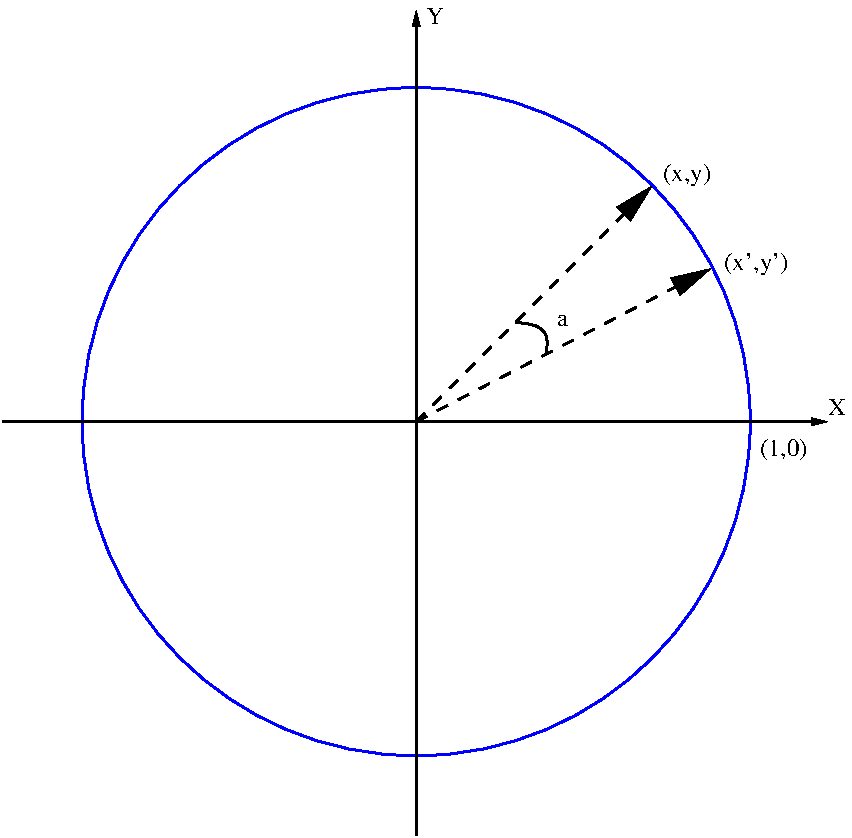
\includegraphics[width=0.5\textwidth]{graphic/CartesianCoordinate.pdf}
\caption{Put All The Pictures Here To Fill The First Page To Test Purpose}
{\small [Rotate from (x, y) to $(x^{'},y^{'})$ via angle of 'a'] }
\label{fig:Cartesian}
\end{center}
\end{figure}


\begin{eqnarray}
V^{'} & = & e^{ja} \times V \\
      & = & [cos(a) + j \times sin(a)] \times (x+j \times y) \\
      & = & x \cdot cos(a)-y \cdot sin(a)+j \cdot [x \cdot sin(a) + y \cdot cos(a) ] 
\label{equ:rotateVector}
\end{eqnarray}

With the help of complex numbers and Euler's identity, the relationship between $V$ and $V^{'}$ could be deduced:
\begin{equation}
V=
\begin{bmatrix}
x^{'} 	\\
y^{'}	\\
\end{bmatrix}
= 
\begin{bmatrix}
	x \cdot cos(a) - y \cdot sin(a)	\\
	y \cdot cos(a) + x \cdot sin(a)	\\
\end{bmatrix}
\label{equ:vectorRotated}
\end{equation}

Equ. \eqref{equ:vectorRotated} could be re-arrange as \eqref{x_cordic1} and \eqref{y_cordic1}.
\begin{align}
 x^{'}		& 	=cos(a) \cdot [x-y \cdot tan(a)]	  \label{x_cordic1}\\
 y^{'}		&	=cos(a) \cdot  [y+x \cdot tan(a)]  \label{y_cordic1}
\end{align}


% Table generated by Excel2LaTeX from sheet 'Sheet4'
\begin{table}[!htbp]
  \centering
  \caption{Value Of $tan(2^{-i})$, i=0, 1, 2, 3...}
    \begin{tabular}{|l|l|l|}
    \toprule
    i     &   $2^{-i}$    & $Degree(Arctan(2^{-i})) $   \\
    \midrule
    0     & 1  & 45 \\
    1     & 0.5  & 26.56505 \\
    2     & 0.25  & 14.03624 \\
    3     & 0.125  & 7.125016 \\
    4     & 0.0625  & 3.576334 \\
    5     & 0.03125  & 1.789911 \\
    6     & 0.015625  & 0.895174 \\
    7     & 0.007813  & 0.447614 \\
    8     & 0.003906  & 0.223811 \\
    9     & 0.001953  & 0.111906 \\
    10    & 0.000977  & 0.055953 \\
    11    & 0.000488  & 0.027976 \\
    12    & 0.000244  & 0.013988 \\
    13    & 0.000122  & 0.006994 \\
    14    & 0.000061  & 0.003497 \\
    15    & 0.000031  & 0.001749 \\
    16    & 0.000015  & 0.000874 \\
    \bottomrule
    \end{tabular}%
  \label{tab:ValueOfTan}%
\end{table}%


\begin{align}
 x_{i+1}	& 	=cos(a_i) \cdot  [x_{i}- y_i \cdot 2^{-i} \cdot d_i]	\label{x_cordic2} \\
y_{i+1}	&	=cos(a_i) \cdot  [y_{i} + x_i \cdot 2^{-i} \cdot d_i]	\label{y_cordic2} \\
cos(\alpha) & = \frac{1}{\sqrt[2]{1+ tan^{2}(\alpha)}}   \label{equ:CosTanRelation}
\end{align}
\\[-11ex] %though this is what I would not recommand, but it's an alternative if you don't have any solution to make the format beauty.
\begin{equation}
K_{i}  =  cos(arctan(2^{-i})) = \frac{1}{\sqrt[2]{1+tan(arctan(2^{-i}))}} = \frac{1}{\sqrt[2]{}1+2^{-2 \cdot i}} \label{equ:Kfactor}\\
\end{equation}
The product of $K_{i}$ represents the so-called $K$ factor (Equ. \ref{equ:Kfactor2})
\begin{equation}
K=\prod K_i = \prod^{n-1}_{i=0} \frac{1}{\sqrt{1+2^{-2 \cdot i}}}
\label{equ:Kfactor2}
\end{equation}

Table \ref{tab:Kfactor} indicates the change of $K$ factor as the iteration increases. It can be noticed that $K$ will reach the limit of $0.607252935$. Hence, The $K$ factor could be calculated in advance and applied elsewhere in the system. A good solution to implement the $K$ factor is to initialize the iterative rotation with a vector of length $\frac{1}{|K|}$ and this will compensate the gain inherent in the CORDIC algorithm.

\input{table/Kfactor_table}

Removing the $K$ factor, Eqn. \eqref{x_cordic2} and \eqref{y_cordic2} turn into the classical CORDIC Equations \eqref{x_cordic3} and \eqref{y_cordic3}.
\begin{align}
 x_{i+1}	&	= [x_{i}- y_i \cdot 2^{-i} \cdot d_i]	\label{x_cordic3}	\\
y_{i+1}	&	=  [y_{i} + x_i \cdot 2^{-i} \cdot d_i]	\label{y_cordic3}
\end{align}

Considering the aim of the CORDIC algorithm is to rotate a vector $V(x,y)$ to unit vector $(1,0)$, the direction of each rotation can be decided by $y_{i+1}$ or the angle accumulator, which is defined as $Z_{i+1}$. Since $y_{i+1}$ would finally be $0$, via Equ. \eqref{y_cordic3}, the direction of rotation could be defined as:
\begin{equation}
d_{i} = \Bigg\{ 
\begin{array}{ccc}
+1 & if &  y_i <  0      	\\
-1 & if &  y_i \ge 0       \\
\end{array}
\label{equ:rotateDirection}
\end{equation}

To be consistent of the definition above, defining the original angle $Z_0$, the angle accumulator can be defined as:
\begin{equation}
Z_{i+1}=  Z_{i} + d_i \cdot arctan(2^{-i})	
\label{equ:AccAngle}
\end{equation}

Another approach to decide the direction of ratation is by judging the current Accumulated Angle $Z_0$. With the definition in Equ. \eqref{equ:AccAngle}, Eqn. \eqref{equ:rotateDirection} could be re-defined as:
\begin{equation}
d_{i} = \Bigg\{ 
\begin{array}{ccccc}
+1 & if &  y_i <  0 & or & Z_i < 0    	\\
-1 & if &  y_i >= 0 & or & Z_i \ge 0   \\
\end{array}
\label{equ:rotateDirection2}
\end{equation}
\\ %I don't know why but this is an example of unbalanced vertical spacing, I have no control over this. Please comment this line and compare the difference if you are interested.
Now, both $y_i$ and $Z_i$ are consistent with the rotation direction $d_i$. The sum of an infinite number of iterative rotation angles would be equal to $-Z_0$ [Equ. \eqref{equ:SumAngle}].
\begin{equation}
Z_{0}= - \sum_{i=0}^{+\infty} d_i \cdot arctan(2^{-i})
\label{equ:SumAngle}
\end{equation}

With Equation \eqref{x_cordic3}, \eqref{y_cordic3},\eqref{equ:AccAngle} and Equation \eqref{equ:rotateDirection2}, the CORDIC algorithm in rotation mode is completely described. Because $arctan(2^0 )=45^{\circ}$  is add/subtract in the 1st iteration, the CORDIC approach is originally applicable for angles within $-\pi /2$ and  $\pi /2$. But trigonometric (sin/cos) is symmetric from quadrant to quadrant. That makes it easy to extend the range to within $0$ and $2\pi$.

Table \ref{tab:WholeCordicProcedure} continues the iterative process.

% Table generated by Excel2LaTeX from sheet 'Sheet4'
\begin{landscape}
%\begin{sidewaystable}[!hbtp]
\begin{table}[!hbtp]
  \caption{The completed procedure of CORDIC iteration}
  \label{tab:WholeCordicProcedure}%
    \begin{tabular}{|l|l|r|r|l|l|l|l|l|}
    \toprule
    \multicolumn{1}{c}{1} & \multicolumn{1}{c}{2} & \multicolumn{1}{c}{3} & \multicolumn{1}{c}{4} & \multicolumn{1}{c}{5} & \multicolumn{1}{c}{6} & 7     & 8     & 9 \\
    \midrule
    Vector Indicator & $X_i$ & $Y_i$ & $d_i$ & $Z_i + d_i \cdot arctan(2^{-i})$ & $\sum_{0}^{i} d_i \cdot arctan(2^{-i})$ & i & $2^{-i}$ & $arctan(2^{-i})$ \\
    \multicolumn{1}{c}{} &       &       &       &       &       &       &       &  \\

%    X0,Y0 & 0.92051 & 0.39073 & -1    & 23.00000 & -45.00000 & 0     & 1.00000 & 45.00000 \\
%    X1,Y1 & 1.31124 & -0.52977 & 1     & -22.00000 & -18.43495 & 1     & 0.50000 & 26.56505 \\
%    X2,Y2 & 1.57612 & 0.12584 & -1    & 4.56505 & -32.47119 & 2     & 0.25000 & 14.03624 \\
%    X3,Y3 & 1.60758 & -0.26819 & 1     & -9.47119 & -25.34618 & 3     & 0.12500 & 7.12502 \\
%    X4,Y4 & 1.64111 & -0.06724 & 1     & -2.34618 & -21.76984 & 4     & 0.06250 & 3.57633 \\
%    X5,Y5 & 1.64531 & 0.03533 & -1    & 1.23016 & -23.55975 & 5     & 0.03125 & 1.78991 \\
%    X6,Y6 & 1.64641 & -0.01609 & 1     & -0.55975 & -22.66458 & 6     & 0.01563 & 0.89517 \\
%    X7,Y7 & 1.64667 & 0.00964 & -1    & 0.33542 & -23.11219 & 7     & 0.00781 & 0.44761 \\
%    X8,Y8 & 1.64674 & -0.00322 & 1     & -0.11219 & -22.88838 & 8     & 0.00391 & 0.22381 \\
%    X9,Y9 & 1.64675 & 0.00321 & -1    & 0.11162 & -23.00029 & 9     & 0.00195 & 0.11191 \\
%    X10,Y10 & 1.64676 & -0.00001 & 1     & -0.00029 & -22.94433 & 10    & 0.00098 & 0.05595 \\
%    X11,Y11 & 1.64676 & 0.00160 & -1    & 0.05567 & -22.97231 & 11    & 0.00049 & 0.02798 \\
%    X12,Y12 & 1.64676 & 0.00080 & -1    & 0.02769 & -22.98630 & 12    & 0.00024 & 0.01399 \\
%    X13,Y13 & 1.64676 & 0.00039 & -1    & 0.01370 & -22.99329 & 13    & 0.00012 & 0.00699 \\
%    X14,Y14 & 1.64676 & 0.00019 & -1    & 0.00671 & -22.99679 & 14    & 6.10E-05 & 0.00350 \\
%    X15,Y15 & 1.64676 & 0.00009 & -1    & 0.00321 & -22.99854 & 15    & 3.05E-05 & 0.00175 \\
%    X16,Y16 & 1.64676 & 0.00004 & -1    & 0.00146 & -22.99941 & 16    & 1.53E-05 & 0.00087 \\
    

    X0,Y0 & \colorbox{green}{0.920505} & \colorbox{green}{0.390731} & -1    & \colorbox{green}{23}    & -45   & 0     & 1     & 45 \\
    X1,Y1 & 1.311235982 & -0.52977372 & 1     & -22   & -18.43494882 & 1     & 0.5   & 26.56505 \\
    X2,Y2 & 1.576122844 & 0.125844266 & -1    & 4.565051177 & -32.47119229 & 2     & 0.25  & 14.03624 \\
    X3,Y3 & 1.607583911 & -0.26818645 & 1     & -9.471192291 & -25.34617594 & 3     & 0.125 & 7.12502 \\
    X4,Y4 & 1.641107217 & -0.06723846 & 1     & -2.346175942 & -21.76984157 & 4     & 0.0625 & 3.57633 \\
    X5,Y5 & 1.64530962 & 0.035330745 & -1    & 1.230158433 & -23.55975218 & 5     & 0.03125 & 1.78991 \\
    X6,Y6 & 1.646413706 & -0.01608518 & 1     & -0.559752175 & -22.66457846 & 6     & 0.015625 & 0.89517 \\
    X7,Y7 & 1.646665037 & 0.009640033 & -1    & 0.335421535 & -23.11219264 & 7     & 0.0078125 & 0.44761 \\
    X8,Y8 & 1.64674035 & -0.00322454 & 1     & -0.112192636 & -22.88838214 & 8     & 0.00390625 & 0.22381 \\
    X9,Y9 & 1.646752945 & 0.003208042 & -1    & 0.111617865 & -23.00028781 & 9     & 0.001953125 & 0.11191 \\
    X10,Y10 & 1.646759211 & -8.27E-06 & 1     & -0.000287813 & -22.94433492 & 10    & 0.000976563 & 0.05595 \\
    X11,Y11 & 1.646759219 & 0.001599891 & -1    & 0.055665079 & -22.97231137 & 11    & 0.000488281 & 0.02798 \\
    X12,Y12 & 1.64676 & 0.00079581 & -1    & 0.027688627 & -22.9862996 & 12    & 0.000244141 & 0.01399 \\
    X13,Y13 & 1.646760195 & 0.000393768 & -1    & 0.0137004 & -22.99329371 & 13    & 0.00012207 & 0.00699 \\
    X14,Y14 & 1.646760243 & 0.000192748 & -1    & 0.006706286 & -22.99679077 & 14    & 6.10E-05 & 0.0035 \\
    X15,Y15 & 1.646760255 & 9.22E-05 & -1    & 0.003209229 & -22.9985393 & 15    & 3.05E-05 & 0.00175 \\
    X16,Y16 & 1.646760257 & 4.20E-05 & -1    & 0.001460701 & \colorbox{red}{-22.99941356} & 16    & 1.53E-05 & 0.00087 \\
    \bottomrule
    \end{tabular}%
           
             {\small [By University Requirement, no text should be allowed here in this landscape table/picture page. \textbf{ DON''T USE sidewaystable from rotating package, it cannot align landscape title to the left binding side.}]}
\end{table}
\end{landscape}



\paragraph{Paragraph Test Example 1}

The structure is directly described by schematics in Figure \ref{IterativeCORDIC}. The branch of $X(i)$ representing the Equation \ref{x_cordic3}, the branch of $Y(i)$ that corresponds to the Equation \ref{y_cordic3}. Equation \ref{equ:AccAngle} is mapped to the 3rd branch with $Z(i)$. Table \ref{tab:WholeCordicProcedure} can be referred to for a better understanding of the whole process. 

\begin{figure}[!htbp]
\begin{center}
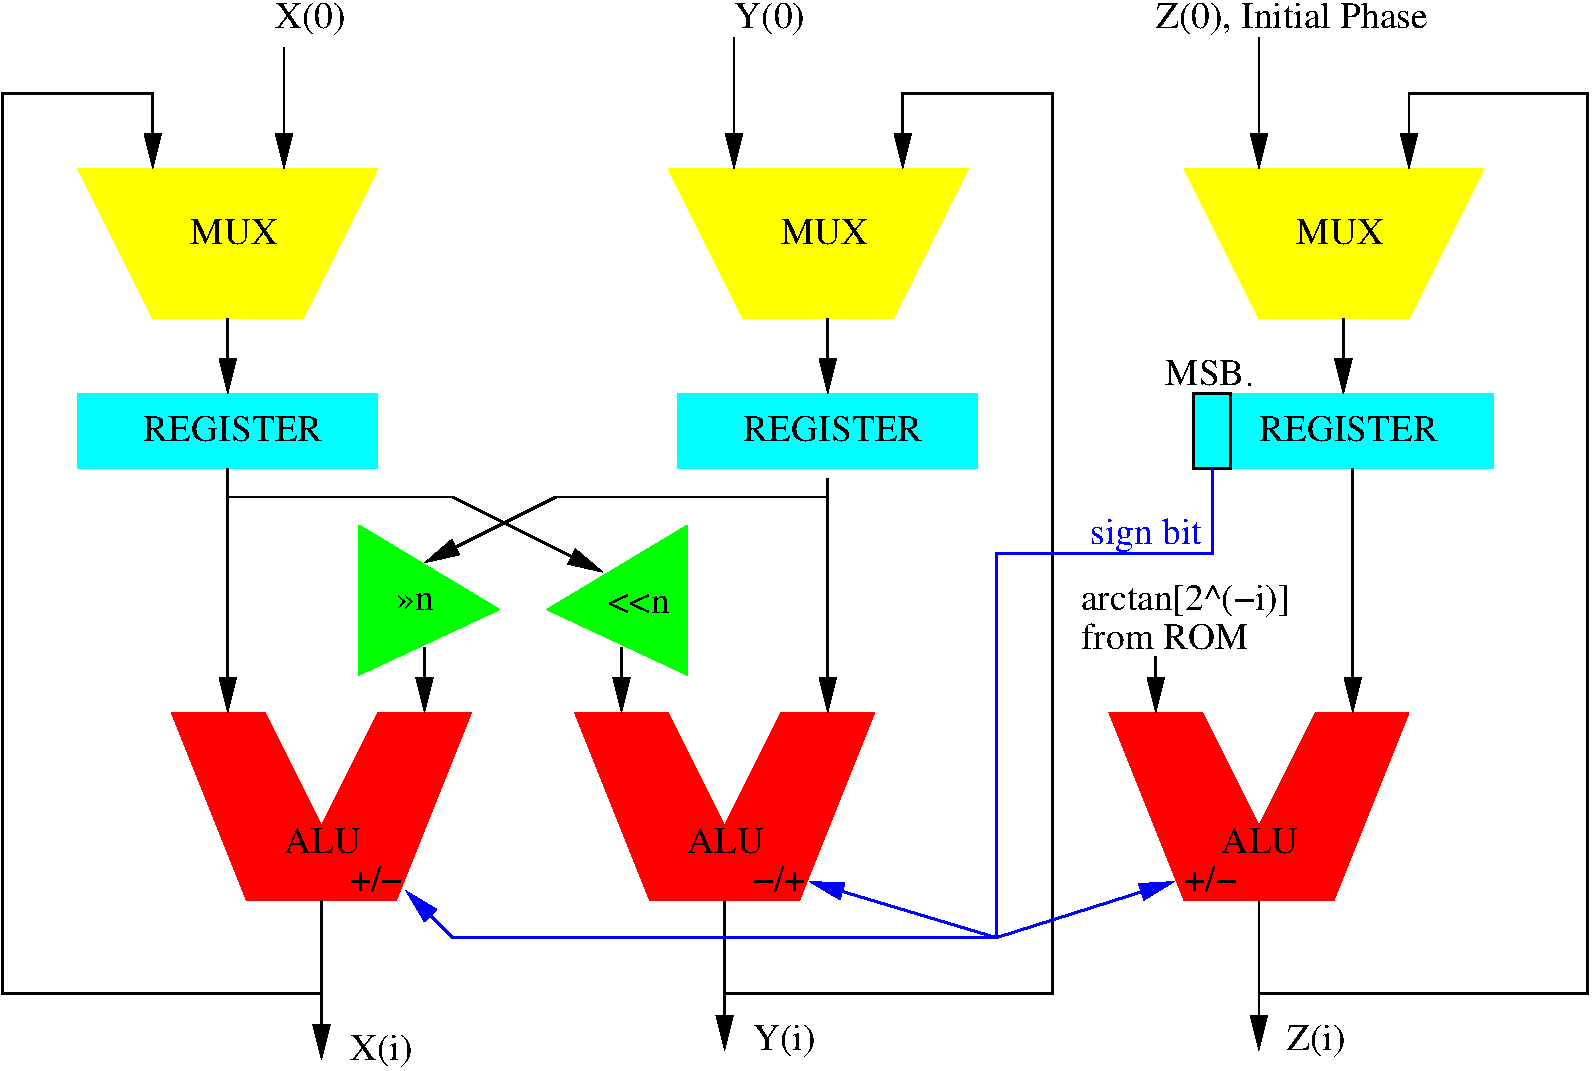
\includegraphics[width=\textwidth]{graphic/BitParallelIterativeCORDIC.pdf}
\caption{Example Of Bit Parallel Iterative CORDIC}
{\small[Picture is from \verb|http://goo.gl/AwCnb|, re-draw for this thesis template]}
\label{IterativeCORDIC}
\end{center}
\end{figure}

The ROM address to obtain $arctan[2^{-i}]$ in the Z branch above.

\paragraph{Paragraph Test Example 2}
Test paragraph without meaningful text. As shown in Figure \ref{fig:UnrollCORDIC}. Several simplifications become possible here.

\begin{figure}[!hbp]
\begin{center}
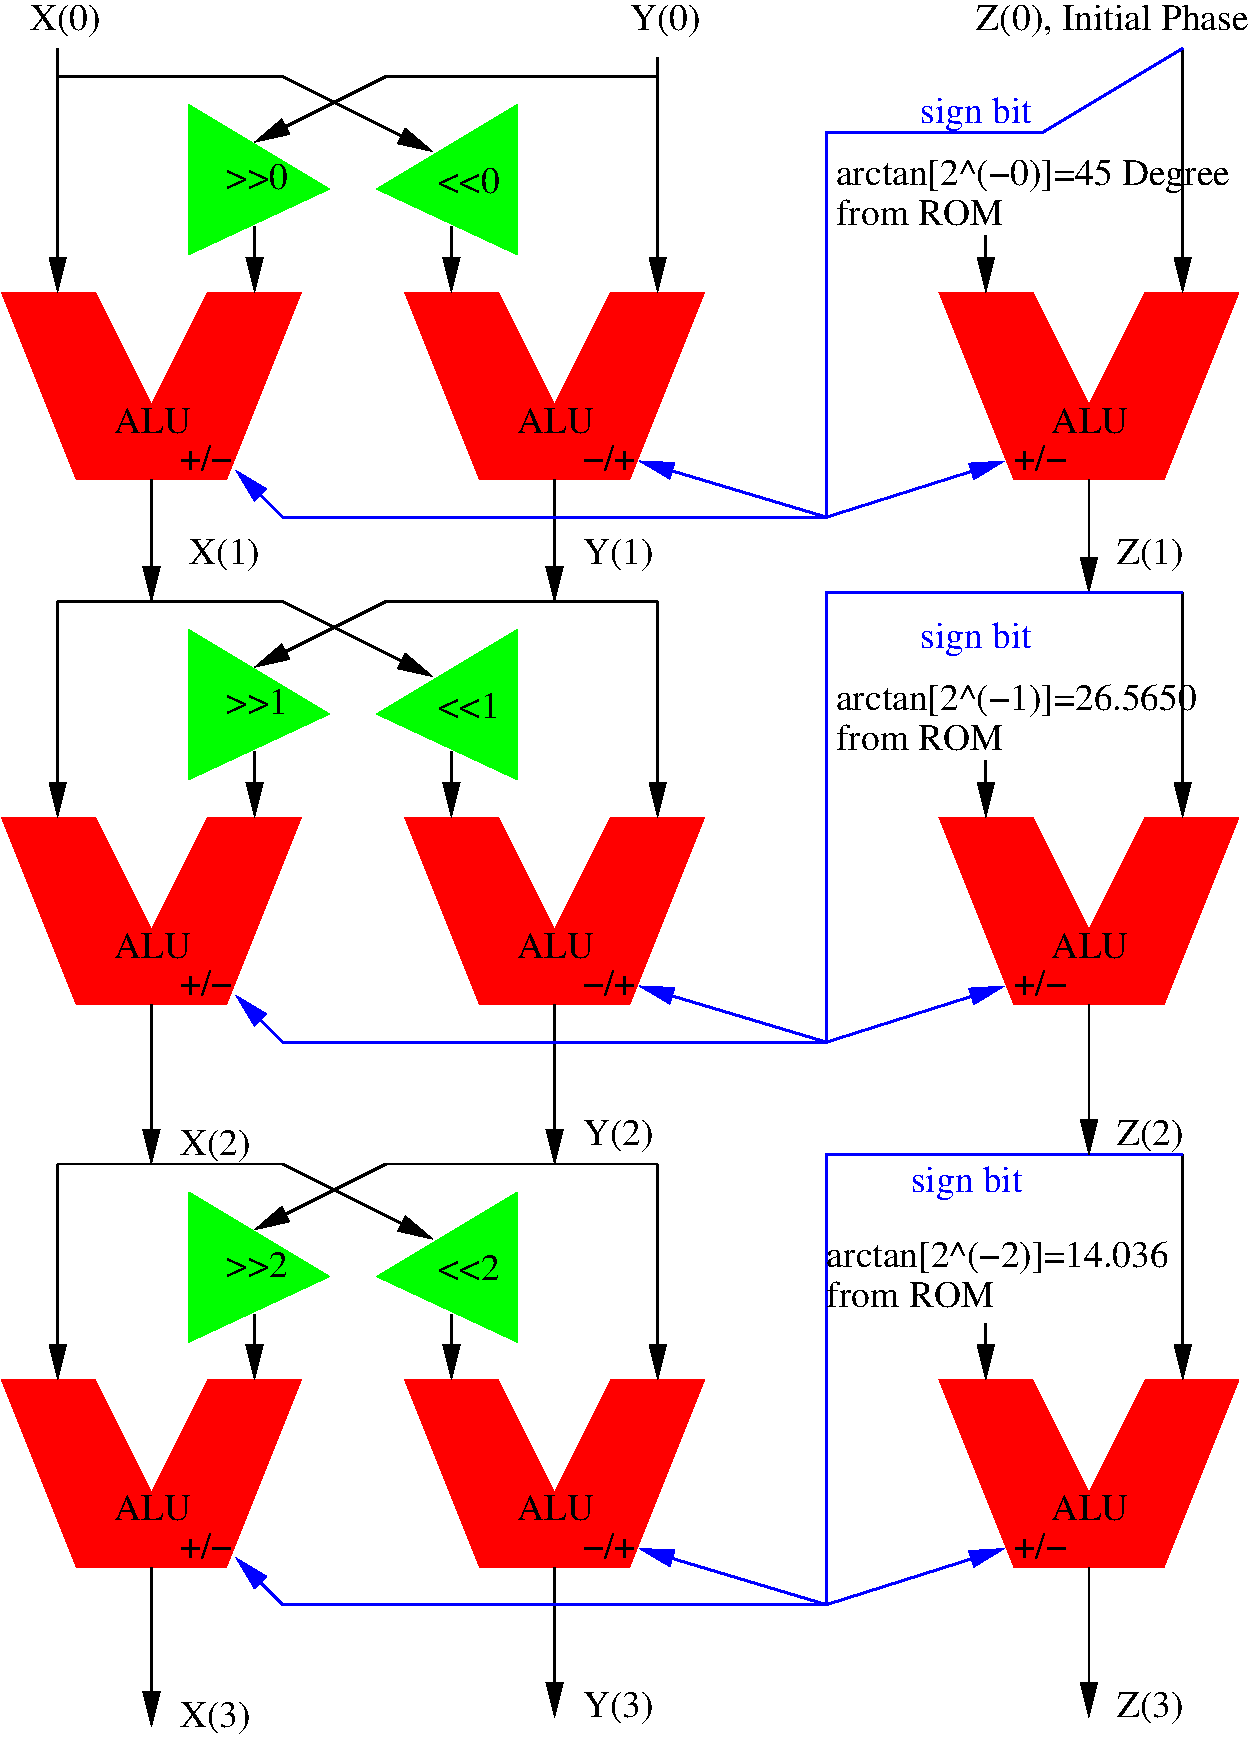
\includegraphics[width=\textwidth]{graphic/BitParallelUnrollCORDIC.pdf}
\caption{Bit Parallel Unrolled CORDIC}
{\small[Picture comes from \verb|http://goo.gl/AwCnb|, re-draw for this thesis template]}
\label{fig:UnrollCORDIC}
\end{center}
\end{figure}


\subsection{Subsection Test Example I Forget}

\begin{figure}[!hbp]
\begin{center}
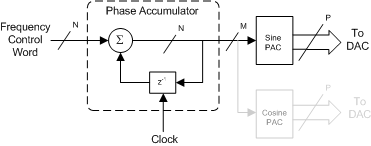
\includegraphics[width=\textwidth]{graphic/Generic_NCO.png}
\caption{Example Picture}
\label{fig:NCO}
\end{center}
\end{figure}


\subsection{Section Summary}

\begin{figure}[!hbpt]
\begin{center}
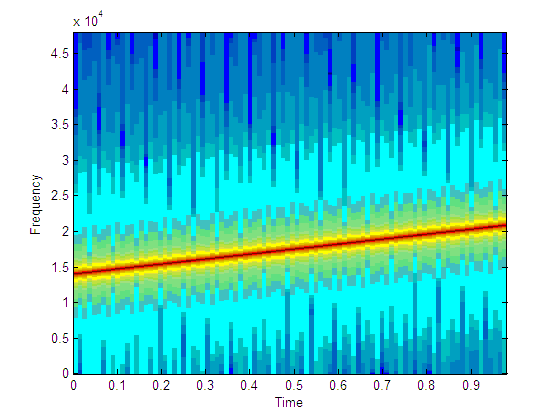
\includegraphics[width=0.8\textwidth]{graphic/AfterDigitalized.png}
\caption{Matlab Output Example}
\label{fig:MatlabChirp}
\end{center}
\end{figure}

\subsubsection{Phase To (X, Y)}
I would recommend to put some text between section title and equation.
\begin{equation}
d_{i} = \Bigg\{ 
\begin{array}{ccc}
+1 & if &  y_i <  \phi      	\\
-1 & if &  y_i \ge \phi       \\
\end{array}
\label{equ:phiRange}
\end{equation}
Test Text between equations. After the specific iteration round is reached, like i = 16, the value in register of X and Y, after multiplication by K factor, are equal to $cos(\phi)$ and $sin(\phi)$. Table \ref{tab:Phase2Cosine} shows the steps in detail for calculating $(cos(\phi) ,sin(\phi))$ from phase $\phi$. In that case, The degree or phase targeted is a \textbf{known} value, which is 23 degree before calculation. The column of 4 is decided by the Equ. \eqref{equ:23Range}.
\begin{equation}
d_{i} = \Bigg\{ 
\begin{array}{ccc}
+1 & if &  y_i <  23      	\\
-1 & if &  y_i \ge 23       \\
\end{array}
\label{equ:23Range}
\end{equation}

\subsubsection{(X, Y) To Phase}
Table \ref{tab:Cosine2Phase} can be referred for this procedure. The only difference from Table \ref{tab:Phase2Cosine} to this is the calculation of $d_i$ is decided by the positive/negative of $y_i$ which shows in Equation \ref{equ:rotateDirection}.
% Table generated by Excel2LaTeX from sheet 'Sheet4'
\begin{landscape}
\begin{table}
  \caption{(X,Y) To Phase CORDIC calculation}
  \label{tab:Cosine2Phase}%
    \begin{tabular}{|l|l|r|r|l|l|l|l|l|}
    \toprule
    \multicolumn{1}{c}{1} & \multicolumn{1}{c}{2} & \multicolumn{1}{c}{3} & \multicolumn{1}{c}{4} & \multicolumn{1}{c}{5} & \multicolumn{1}{c}{6} & 7     & 8     & 9 \\
    \midrule
    Vector Indicator & $X_i$ & $Y_i$ & $d_i$ & $Z_i + d_i \cdot arctan(2^{-i})$ & $\sum_{0}^{i} d_i \cdot arctan(2^{-i})$ & i & $2^{-i}$ & $arctan(2^{-i})$ \\
    \multicolumn{1}{c}{} &       &       &       &       &       &       &       &  \\
    X0,Y0 & \colorbox{green}{0.920505} & \colorbox{green}{0.390731} & -1    & 23.000 & -45   & 0     & 1     & 45.00000 \\
    X1,Y1 & 1.311235982 & -0.52977372 & 1     & -22   & -18.43494882 & 1     & 0.5   & 26.56505 \\
    X2,Y2 & 1.576122844 & 0.125844266 & -1    & 4.565051177 & -32.47119229 & 2     & 0.25  & 14.03624 \\
    X3,Y3 & 1.607583911 & -0.26818645 & 1     & -9.471192291 & -25.34617594 & 3     & 0.125 & 7.12502 \\
    X4,Y4 & 1.641107217 & -0.06723846 & 1     & -2.346175942 & -21.76984157 & 4     & 0.0625 & 3.57633 \\
    X5,Y5 & 1.64530962 & 0.035330745 & -1    & 1.230158433 & -23.55975218 & 5     & 0.03125 & 1.78991 \\
    X6,Y6 & 1.646413706 & -0.01608518 & 1     & -0.559752175 & -22.66457846 & 6     & 0.015625 & 0.89517 \\
    X7,Y7 & 1.646665037 & 0.009640033 & -1    & 0.335421535 & -23.11219264 & 7     & 0.0078125 & 0.44761 \\
    X8,Y8 & 1.64674035 & -0.00322454 & 1     & -0.112192636 & -22.88838214 & 8     & 0.00390625 & 0.22381 \\
    X9,Y9 & 1.646752945 & 0.003208042 & -1    & 0.111617865 & -23.00028781 & 9     & 0.001953125 & 0.11191 \\
    X10,Y10 & 1.646759211 & -8.2721E-06 & 1     & -0.000287813 & -22.94433492 & 10    & 0.000976563 & 0.05595 \\
    X11,Y11 & 1.646759219 & 0.001599891 & -1    & 0.055665079 & -22.97231137 & 11    & 0.000488281 & 0.02798 \\
    X12,Y12 & 1.64676 & 0.00079581 & -1    & 0.027688627 & -22.9862996 & 12    & 0.000244141 & 0.01399 \\
    X13,Y13 & 1.646760195 & 0.000393768 & -1    & 0.0137004 & -22.99329371 & 13    & 0.00012207 & 0.00699 \\
    X14,Y14 & 1.646760243 & 0.000192748 & -1    & 0.006706286 & -22.99679077 & 14    & 6.10352E-05 & 0.00350 \\
    X15,Y15 & 1.646760255 & 9.22377E-05 & -1    & 0.003209229 & -22.9985393 & 15    & 3.05176E-05 & 0.00175 \\
    X16,Y16 & 1.646760257 & 4.19826E-05 & -1    & 0.001460701 & \colorbox{red}{-22.99941356} & 16    & 1.52588E-05 & 0.00087 \\
    \bottomrule
    \end{tabular}%

{\small [By University Requirement, no text should be allowed here in this landscape table/picture page. \textbf{ DON''T USE sidewaystable from rotating package, it cannot align landscape title to the left binding side.]}}
\end{table}
\end{landscape}
 
% Table generated by Excel2LaTeX from sheet 'Sheet4'
%\begin{sidewaystable}[!hbtp]
\begin{landscape}
\begin{table}
\captionsetup{list=off}	%disable lof display this figure name as continued
  \caption{Phase to (X,Y) CORDIC calculation}
  \label{tab:Phase2Cosine}%
    \begin{tabular}{|l|l|r|r|l|l|l|l|l|}
    \toprule
    \multicolumn{1}{c}{1} & \multicolumn{1}{c}{2} & \multicolumn{1}{c}{3} & \multicolumn{1}{c}{4} & \multicolumn{1}{c}{5} & \multicolumn{1}{c}{6} & 7     & 8     & 9 \\
    \midrule
    Vector Indicator & $X_i$ & $Y_i$ & $d_i$ & $Z_i + d_i \cdot arctan(2^{-i})$ & $\sum_{0}^{i} d_i \cdot arctan(2^{-i})$ & i & $2^{-i}$ & $arctan(2^{-i})$ \\
    \multicolumn{1}{c}{} &       &       &       &       &       &       &       &  \\

    X0,Y0 & \colorbox{green}{1}     & \colorbox{green}{0}     & 1     & \colorbox{green}{0}     & 45    & 0     & 1     & 45 \\
    X1,Y1 & 1     & 1     & -1    & 45    & 18.4349488 & 1     & 0.5   & 26.56505 \\
    X2,Y2 & 1.5   & 0.5   & 1     & 18.43495 & 32.4711923 & 2     & 0.25  & 14.03624 \\
    X3,Y3 & 1.375 & 0.875 & -1    & 32.47119 & 25.3461759 & 3     & 0.125 & 7.125016 \\
    X4,Y4 & 1.484375 & 0.703125 & -1    & 25.34618 & 21.7698416 & 4     & 0.0625 & 3.576334 \\
    X5,Y5 & 1.52832 & 0.610352 & 1     & 21.76984 & 23.5597522 & 5     & 0.03125 & 1.789911 \\
    X6,Y6 & 1.509247 & 0.658112 & -1    & 23.55975 & 22.6645785 & 6     & 0.015625 & 0.895174 \\
    X7,Y7 & 1.51953 & 0.63453 & 1     & 22.66458 & 23.1121926 & 7     & 0.0078125 & 0.447614 \\
    X8,Y8 & 1.514573 & 0.646401 & -1    & 23.11219 & 22.8883821 & 8     & 0.0039063 & 0.223811 \\
    X9,Y9 & 1.517098 & 0.640485 & 1     & 22.88838 & 23.0002878 & 9     & 0.0019531 & 0.111906 \\
    X10,Y10 & 1.515847 & 0.643448 & -1    & 23.00029 & 22.9443349 & 10    & 0.0009766 & 0.055953 \\
    X11,Y11 & 1.516475 & 0.641967 & 1     & 22.94433 & 22.9723114 & 11    & 0.0004883 & 0.027976 \\
    X12,Y12 & 1.516162 & 0.642708 & 1     & 22.97231 & 22.9862996 & 12    & 0.0002441 & 0.013988 \\
    X13,Y13 & 1.516005 & 0.643078 & 1     & 22.9863 & 22.9932937 & 13    & 0.0001221 & 0.006994 \\
    X14,Y14 & 1.515926 & 0.643263 & 1     & 22.99329 & 22.9967908 & 14    & 6.104E-05 & 0.003497 \\
    X15,Y15 & 1.515887 & 0.643356 & 1     & 22.99679 & 22.9985393 & 15    & 3.052E-05 & 0.001749 \\
    X16,Y16 & \colorbox{red}{1.515867} & \colorbox{red}{0.643402} & 1     & 22.99854 & 22.9994136 & 16    & 1.526E-05 & 0.000874 \\
    \bottomrule
    \end{tabular}%

{\small [By University Requirement, no text should appear here in this landscape table/picture page]}
\end{table}
\end{landscape}
%0.607252


% Table generated by Excel2LaTeX from sheet 'Sheet5'
\begin{landscape}
\begin{table}[!hbtp]
  \centering
  \caption{Phase Control Word}
  \label{tab:exFreqControl}%
    \begin{tabular}{|c|c|c|c|c|c|c|c|c|c|c|c|c|c|c|c|c|c|}
    \toprule
          &       & \multicolumn{16}{|c|}{Phase Control Word(Binary)}                                                                            \\
    \midrule
    Frequency & Phase  & Bit  & Bit  & Bit & Bit  & Bit  & Bit & Bit & Bit  & Bit & Bit & Bit  & Bit  & Bit  & Bit  & Bit  & Bit  \\
    & Control Word & 15 &   14 &   13 &   12 &   11 &   10 &   9 &   8 &   7 &   6 &   5 &   4 &   3 &   2 &   1 &   0 \\
\hline
    48000 & 16384 & 0     & 1     & 0     & 0     & 0     & 0     & 0     & 0     & 0     & 0     & 0     & 0     & 0     & 0     & 0     & 0 \\
    1000  & 341   & 0     & 0     & 0     & 0     & 0     & 0     & 0     & 1     & 0     & 1     & 0     & 1     & 0     & 1     & 0     & 1 \\
    8000  & 2731  & 0     & 0     & 0     & 0     & 1     & 0     & 1     & 0     & 1     & 0     & 1     & 0     & 1     & 0     & 1     & 1 \\
    14000 & 4779  & 0     & 0     & 0     & 1     & 0     & 0     & 1     & 0     & 1     & 0     & 1     & 1     & 1     & 1     & 1     & 1 \\
    21000 & 7168  & 0     & 0     & 0     & 1     & 1     & 1     & 0     & 0     & 0     & 0     & 0     & 0     & 0     & 0     & 0     & 0 \\
    \bottomrule
    \end{tabular}%
    
        [{\small By University Requirement, no text should be allowed here in this landscape table/picture page. \textbf{ DON''T USE sidewaystable from rotating package, it cannot align landscape title to the left binding side.}}]
\end{table}
\end{landscape}


A simple paragraph of Verilog code is below in verbatim.
%\textcolor{blue}{
\begin{verbatim}
Always@(posedge LRCK)
        Begin
        	Counter = Counter + 1
        	If (Counter == 40)
        	Begin
         		Counter = 0
	        	Phase_control_word = Phase_Control_word + 1
         		If (phase_control_word >= 7168)
         		Begin
	         		Phase_control_word =4778
		        end
        	end
        end
\end{verbatim}

\section{Section Test Example 3}
Test section for toc display only.

\subsection{Subsection Test 1}
Test subsection for toc display only.

\subsection{Subsection Test 2}
Test subsection for toc display only.

\subsection{Subsection Test 3}

Test subsection for toc display only.

\subsection{Subsection Test 4}

Test subsection for toc display only.

\section{Section Test Example 4}
Test subsection for toc display only.

\begin{figure}[!hbp]
\begin{center}
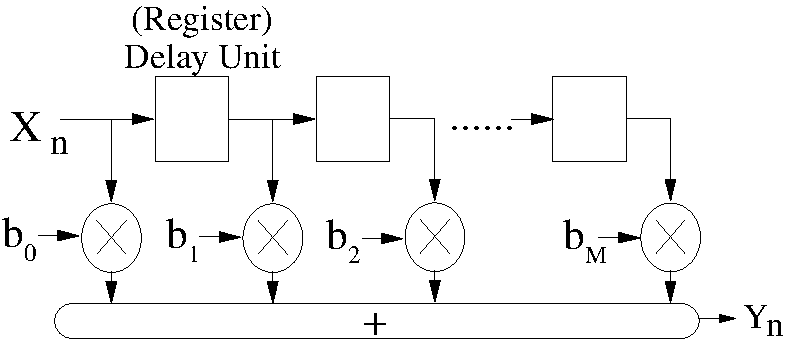
\includegraphics[width=0.6\textwidth]{graphic/FIR_Implementation.pdf}
\caption{Example of FIR Filter}
\label{fig:genFIR}
[Test Picture for lof display purpose only.]
\end{center}
\end{figure}


\begin{figure}[!hbp]
\begin{center}
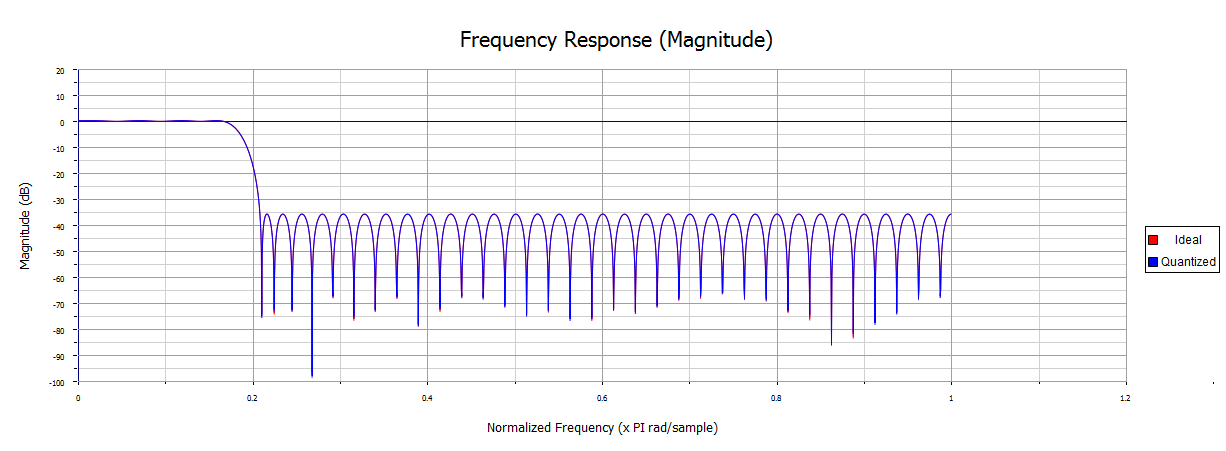
\includegraphics[width=0.8\textwidth]{graphic/LowPass_Filter_Design.PNG}
\caption{Low Pass FIR Filter Spectrum Characterization}
\label{fig:lowpass}
{\small h=firpm(80, [0 8 10 48]/48, [1 1 0 0]); [Test Picture for lof display purpose only.]}
\end{center}
\end{figure}

